% Modello di lucidi per la presentazione di una tesi.
% Collaudato sia con LaTeX che con pdfLaTeX.
% Scritto da Gianluca Gorni.
% Versione: 9 novembre 2006

\documentclass[a4,portrait,italian]{seminar}

\usepackage[latin1]{inputenc}
\usepackage{babel}

\usepackage{uniudlucidi}

% Due opzioni della classe "seminar":
\slideframe{none} % lucidi senza cornice
\raggedslides[1cm] % margine destro elastico

%\usepackage{graphicx} % gia' caricato da uniudlucidi
\graphicspath{{./figure/}}

%\usepackage{hyperref} % gia' caricato da uniudlucidi
\hypersetup{pdftitle={La mia tesi di Matematica},
pdfauthor={Giovanna Tesista},
pdfsubject={Esempio di lucidi per la presentazione di una Tesi di Laurea},
pdfkeywords={LaTeX lucidi presentazione}} % Queste informazioni non vengono stampate, ma sono conservate nel documento pdf (premere command-D per vederle sotto AdobeReader/AcrobatReader). Tornano buone a scopi archivistici.

\usepackage{amsmath,amsfonts,amssymb,amsthm}
\newcommand{\Z}{\mathbb{Z}}
\newcommand{\R}{\mathbb{R}}
\newcommand{\N}{\mathbb{N}}

%\usepackage{color} % gia' caricato da uniudlucidi
\newcommand{\nero}[1]{\textcolor{black}{#1}}
\newcommand{\rosso}[1]{\textcolor{red}{#1}}
\definecolor{darkgreen}{RGB}{51,102,0}
\newcommand{\verdescuro}[1]{\textcolor{darkgreen}{#1}}
\newcommand{\blu}[1]{\textcolor{blue}{#1}}
\definecolor{ocra}{rgb}{.45,.24,.1}
\newcommand{\ocra}[1]{\textcolor{ocra}{#1}}
\newcommand{\sfondogiallo}[1]{\colorbox{yellow}{#1}}
\newcommand{\displaysfondogiallo}[1]{\begin{center}%
  \sfondogiallo{$\displaystyle{#1}$}\end{center}}

% Stili di colorazione degli enunciati:
\newtheoremstyle{Ocra}% name
  {9pt}%      Space above
  {9pt}%      Space below
  {\bfseries\slshape\color{ocra}}% Body font
  {\parindent}%         Indent amount
  {\bfseries\color{black}}% Thm head font
  {.}%        Punctuation after thm head
  {1em}% Space after thm head: \newline = linebreak
  {}%         Thm head spec
\newtheoremstyle{Blu}% name
  {9pt}%      Space above
  {9pt}%      Space below
  {\bfseries\slshape\color{blue}}% Body font
  {\parindent}%         Indent amount
  {\bfseries\color{black}}% Thm head font
  {.}%        Punctuation after thm head
  {1em}% Space after thm head: \newline = linebreak
  {}%         Thm head spec
\newtheoremstyle{Verde}% name
  {9pt}%      Space above
  {9pt}%      Space below
  {\normalfont\color{darkgreen}}% Body font
  {\parindent}%         Indent amount
  {\itshape\color{black}}% Thm head font
  {.}%        Punctuation after thm head
  {1em}% Space after thm head: \newline = linebreak
  {}%         Thm head spec

% Associare gli stili ai diversi enunciati:

\theoremstyle{Ocra}
\newtheorem{teorema}{Teorema}

\theoremstyle{Blu}
\newtheorem{proposizione}{Proposizione}

\theoremstyle{Verde}
\newtheorem{definizione}{Definizione}

% Informazioni per l'intestazione:

\titolo{La mia tesi\\ di Matematica}
\laureanda{Giovanna Laura\\ Tesista}
% \laureando{Giovanni Tesista}
\corsodilaurea{Matematica}
% \corsodilaureatriennale{Informatica}
% \corsodilaureaspecialistica{Fisica Computazionale}
\relatore[Prof.]{Tal dei Tali}
% \correlatore[Prof.]{Talaltro dei Tali}
\data{3 novembre 2003}
% \facolta{Scienze MM. FF. NN.} % default
\dedica{Ai miei genitori\\
    per non avermi tagliato i viveri}
% La dedica e' facoltativa. Si puo' omettere.

% Intestazione: questi sono i colori di default:
% \coloreTitolo{blue}
% \coloreAutori{black}
% \coloreRestoIntestazione{ocra}

\begin{document}

\maketitle

%%%%%%%%%%%%%%%%%%%%%%%%%%%%%%%%%%%%%%%%%%%%%%%%%%%%%%%%%%%%
\begin{slide*}

\section{\texorpdfstring{``Seminar''}{"Seminar"}}

Questi lucidi usano la classe \LaTeX{} \rosso{\texttt{seminar}}, che \`e descritta in dettaglio nel documento (vecchiotto)

\begin{center}
{\tiny
\url{http://tex.loria.fr/services/tex/classes/sem-user.pdf}
}\end{center}

Per esempio,

\begin{itemize}

\item lucidi \rosso{in piedi} (``portrait'') come questi, si fanno con\newline {\color{blue}\verb!\begin{slide*} ... \end{slide*}!}

\item un lucido \rosso{coricato} (``landscape'') si fa con\newline {\color{blue}\verb!\begin{slide} ... \end{slide}!}

\end{itemize}

\end{slide*}
%%%%%%%%%%%%%%%%%%%%%%%%%%%%%%%%%%%%%%%%%%%%%%%%%%%%%%%%%%%
\begin{slide*}

\section{Stampa}

Quando si stampano dei lucidi a colori, bisogna stare attenti a usare lucidi adatti al proprio tipo di stampanti:

\begin{itemize}

\item ci sono lucidi fatti per le stampanti a \rosso{getto d'inchiostro} (inchiostro liquido)

\item e lucidi per le fotocopiatrici e stampanti laser (inchiostro in polvere).

\end{itemize}

L'inchiostro liquido si sbava sui lucidi sbagliati. Sul mercato ci sono anche lucidi double-face.

Esempi di colori: \rosso{rosso}, \verdescuro{verde scuro}, \ocra{ocra}, \blu{blu}.

I~colori chiari, come il \textcolor{green}{verde chiaro} tendono a essere poco leggibili. Il giallo pu\`o andar bene come \sfondogiallo{sfondo}.

\end{slide*}
%%%%%%%%%%%%%%%%%%%%%%%%%%%%%%%%%%%%%%%%%%%%%%%%%%%%%%%%%%%%
\begin{slide*}

\section{Pitagora}

\begin{definizione}
Dicesi \rosso{triangolo rettangolo} ogni triangolo che ha un angolo retto.
\end{definizione}

\begin{teorema}[di Pitagora]
In un triangolo rettangolo, la somma dei quadrati costruiti sui cateti \`e uguale al quadrato costruito sull'ipotenusa.
\end{teorema}

\begin{center}
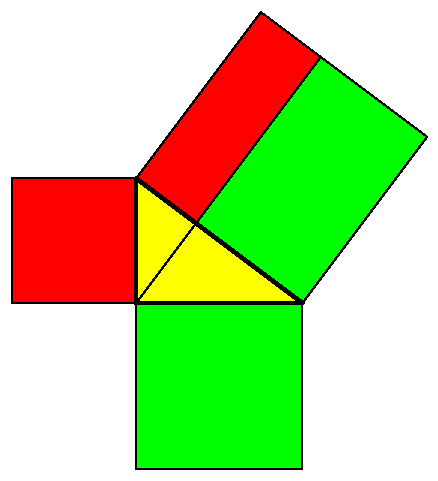
\includegraphics[width=100pt]{pitagora3}
\end{center}

\end{slide*}
%%%%%%%%%%%%%%%%%%%%%%%%%%%%%%%%%%%%%%%%%%%%%%%%%%%%%%%%%
\begin{slide*}

\section{Varie ed eventuali}

\begin{proposizione}
Se questo, allora quello.
\end{proposizione}

\begin{proof}
Per esercizio.
\end{proof}

Una \sfondogiallo{parola} evidenziata con sfondo giallo. Anche una formula:
\displaysfondogiallo{a^2+b^2=c^2.}

Lettere a diversi colori:
\begin{equation*}
  \int \rosso{f}'\bigl(\verdescuro{g}(x)\bigr)
  \verdescuro{g}'(x)\,dx=
  \textcolor{red}{f}\bigl(\verdescuro{g}(x)\bigr)\,.
\end{equation*}

\end{slide*}

%%%%%%%%%%%%%%%%%%%%%%%%%%%%%%%%%%%%%%%%%%%%%%%%%%%%%%%%%
% Chi non vuole il lucido finale, usi
% \renewcommand{\lucidofinale}{}

\end{document}